% Provenance (never printed): old premiere S material on the formation of fossil
% fuels (preserved organic matter, burial, oil window, migration, trap, coal).
% Burial history of the invented Merrow Basin from figdata/grade-11/oil_window.py
% (constant geotherm, no compaction). Rifts and passive margins after the USGS
% West-Central Coastal Province fact sheet (2023-3028). Folds are defined in
% g12.02 mountain-building (Sync 0): the anticline is told in prose here, never
% defined. Sedimentary basins compared, diagenesis: Year 1/2.
\chapter{कोयले, तेल और गैस का भूविज्ञान}\label{ch:g11:fossil-fuel-geology}

पेंसिल्वेनिया की एक पुरानी \omterm{def:g11:fossil-fuel-geology:coal}{कोयला-खान} से लिए गए काले शेल की एक पटिया पर
फ़र्न जैसे पौधों की पत्तियाँ हैं, चपटी और गहरी चट्टान पर चाँदी जैसी। वे
तीन सौ मिलियन वर्ष से भी पहले, कार्बोनिफ़ेरस कल्प में, एक दलदल में उगी थीं;
सड़ने से पहले दब जाने के कारण उन्होंने अपनी आकृति बनाए रखी, और
दलदल के पौधों का कार्बन \omterm{def:g11:fossil-fuel-geology:coal}{कोयला} बन गया। तेल और गैस, जो आज समुद्र में दूर
प्लेटफ़ॉर्मों से निकाले जाते हैं, का मूल भी इसी प्रकार का है: जीवों के
अवशेष जो सड़ने से बच गए और फिर दबकर गरम हुए। यह अध्याय
दबे हुए इस कार्बन का पीछा दलदल और समुद्री तल से \omterm{def:g11:fossil-fuel-geology:coal}{कोयले} की परत
और तेल-क्षेत्र तक करता है।
% ledger: photo:g11-fossil-plants, ics:base.Carboniferous, ics:base.Permian, earle:coal-formation, earle:organic-preservation

\begin{omfigure}
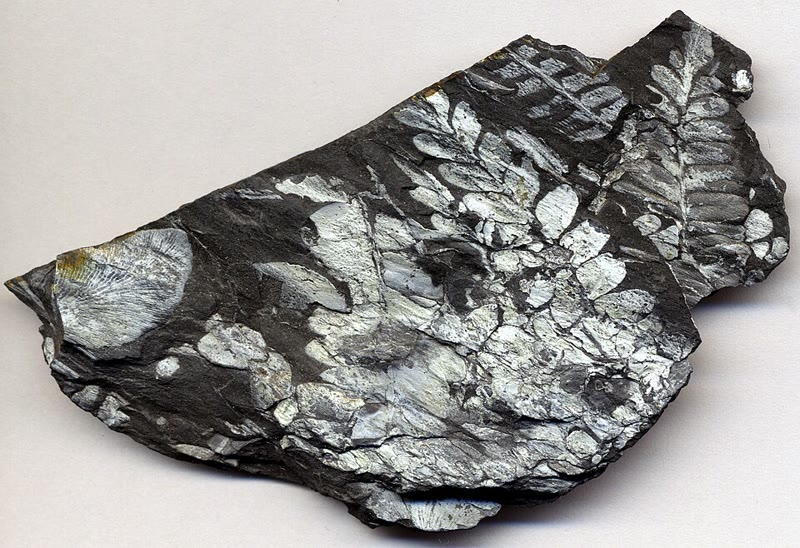
\includegraphics[height=4.4cm]{images/book2/g11-stjohn-fossil-plants.jpg}\hspace{0.03\linewidth}%
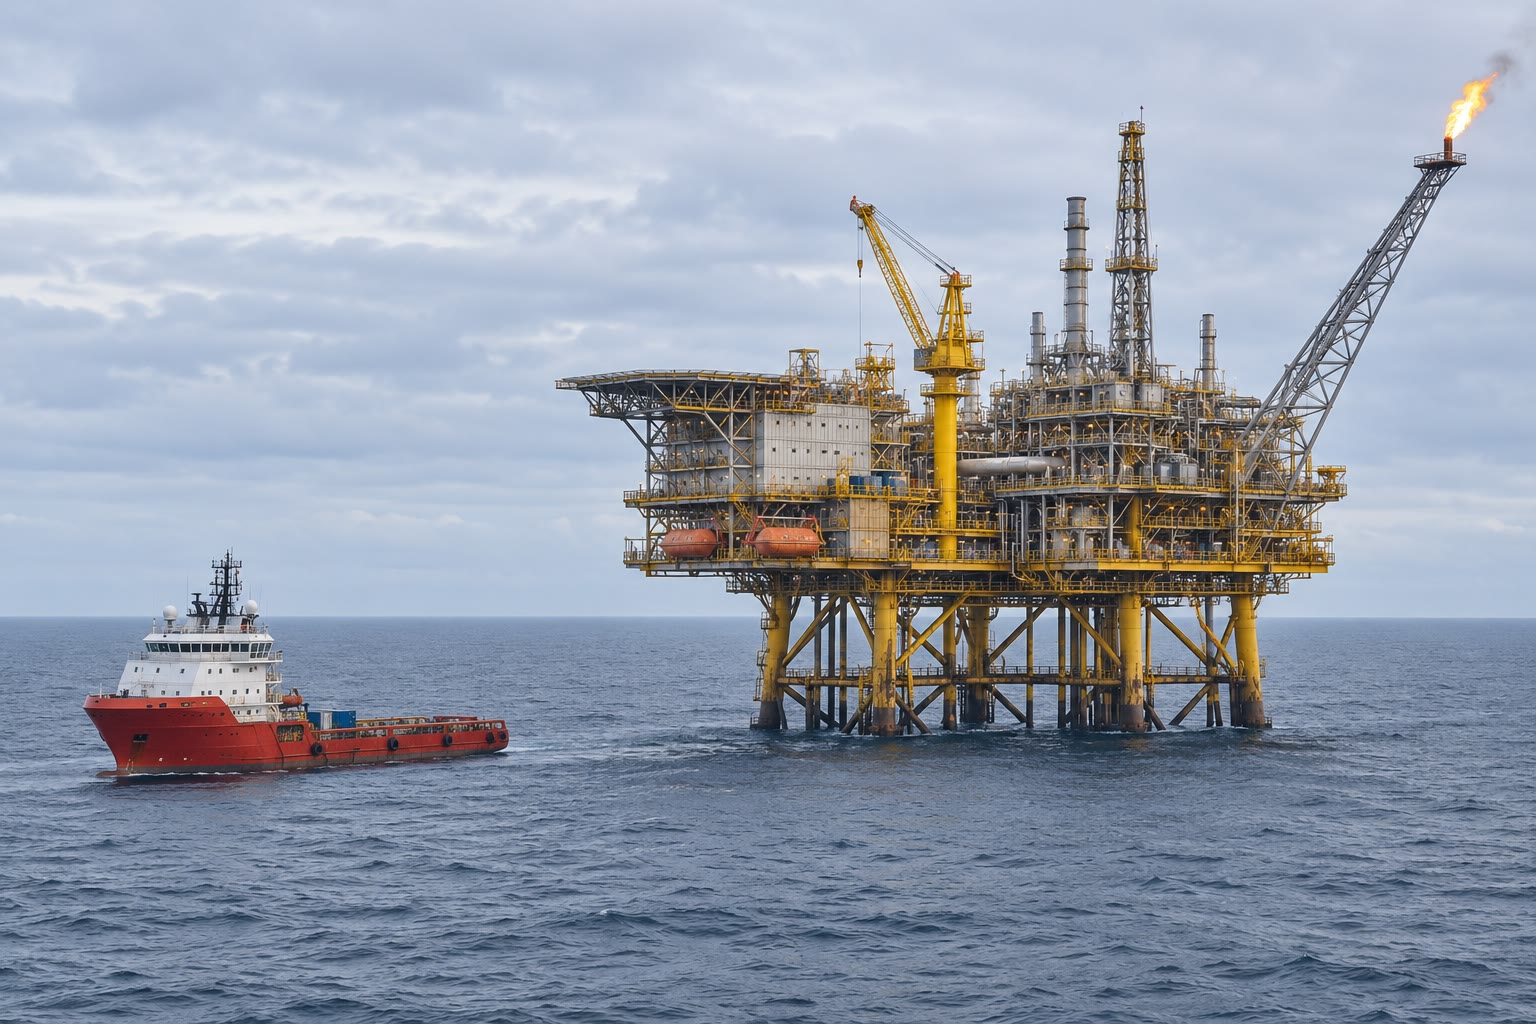
\includegraphics[height=4.4cm]{images/book2/ai/g11-offshore-platform.jpg}

{\small बाएँ: एक पुरानी \omterm{def:g11:fossil-fuel-geology:coal}{कोयला-खान} से कार्बन-समृद्ध शेल में जीवाश्म पौधों की
पत्तियाँ, पेंसिल्वेनिया, कार्बोनिफ़ेरस; पटिया लगभग \qty{10}{cm} चौड़ी है।
फ़ोटो जेम्स सेंट~जॉन (CC~BY~2.0)। दाएँ: समुद्र में तेल और गैस उत्पादन का एक
प्लेटफ़ॉर्म (AI चित्र)।}
\end{omfigure}
% ledger: photo:g11-fossil-plants

\begin{recall}
\omterm{def:g11:fossil-fuel-geology:coal}{कोयला}, तेल और प्राकृतिक गैस जीवाश्म ईंधन हैं: तेल और गैस
हाइड्रोकार्बनों के मिश्रण हैं, जो कार्बन और हाइड्रोजन के यौगिक हैं, और जीवाश्म ईंधन जलाने से
ऊर्जा और कार्बन डाइऑक्साइड मुक्त होती है (रसायन की पुस्तकें)। पौधे और शैवाल
प्रकाशसंश्लेषण द्वारा कार्बन डाइऑक्साइड और पानी से कार्बनिक पदार्थ बनाते हैं (जीव-विज्ञान
की पुस्तकें)। \omterm{def:g11:fossil-fuel-geology:coal}{कोयला}, तेल और गैस अवसादों में दबे कार्बनिक पदार्थ से आते हैं,
और वे अवसादी चट्टानों में संचित होते हैं (पुस्तक 1, कक्षा 9)। चट्टान
सरंध्र होती है जब उसमें खाली जगहें हों, पारगम्य जब पानी उसमें से होकर बह सके
(पुस्तक 1, कक्षा 6)। \omterm{def:g11:lithosphere-asthenosphere:geotherm}{भूतापीय वक्र} के अनुदिश तापमान गहराई के साथ बढ़ता है,
पहले कुछ किलोमीटरों में प्रति किलोमीटर 25 से \qty{30}{\degreeCelsius}
(\cref{ch:g11:lithosphere-asthenosphere})।
\end{recall}
% ledger: usgs:gradient-29, earle:organic-preservation

\section{कार्बनिक पदार्थ का संरक्षण}

अधिकांश कार्बनिक पदार्थ कभी ईंधन नहीं बनता। किसी मृत पत्ती या मृत शैवाल को
जंतु और जीवाणु खा जाते हैं या वह हवा की ऑक्सीजन से अभिक्रिया करता है: कुछ
हफ़्तों या वर्षों में उसका कार्बन कार्बन डाइऑक्साइड के रूप में वायुमंडल में लौट जाता है।
कार्बनिक पदार्थ केवल वहीं बचता है जहाँ वह ऑक्सीजन से कटा हो --- किसी
ठहरे दलदल की तली पर, या किसी ऐसे समुद्री तल या झील-तल पर जिसके पानी में
कोई ऑक्सीजन न हो। वहाँ और अवसाद के नीचे दबकर वह दसियों या
सैकड़ों मिलियन वर्षों तक बचा रह सकता है।
% ledger: earle:organic-preservation

\omterm{def:g11:fossil-fuel-geology:coal}{कोयला} ज़्यादातर उन स्थलीय पौधों से आता है जो दलदलों में ढेर हुए। तेल और गैस
ज़्यादातर समुद्र के सूक्ष्म शैवालों और दूसरे प्लवकों से आते हैं: जहाँ
सतही जल बहुत उत्पादक होते हैं, वहाँ मृत प्लवक समुद्री तल पर
इतनी तेज़ी से बरसते हैं कि उनमें से कुछ सड़ने से बच जाते हैं, और वे कीचड़ में दब जाते हैं।
% ledger: earle:coal-formation, earle:oil-window

\begin{definition}[स्रोत चट्टान; केरोजन]\label{def:g11:fossil-fuel-geology:source-rock}
\emph{केरोजन}\index{केरोजन} किसी अवसादी चट्टान में बिखरा कार्बनिक पदार्थ है,
ऐसे छोटे कणों में जो कार्बनिक विलायकों में नहीं घुलते।
\emph{स्रोत चट्टान}\index{स्रोत चट्टान} केरोजन से समृद्ध वह अवसादी चट्टान है
जिसमें दबने और गरम होने पर तेल और गैस बनते हैं।
\end{definition}
% ledger: peters08:kerogen, earle:migration-traps

अधिकांश \omterm{def:g11:fossil-fuel-geology:source-rock}{स्रोत चट्टानें} शेल और पंकाश्म हैं, जो कार्बनिक पदार्थ से समृद्ध कीचड़ के रूप में
जमे थे। सतह के पास उनका \omterm{def:g11:fossil-fuel-geology:source-rock}{केरोजन} ठोस रहता है: ऑक्सीजन के बिना
रहने वाले जीवाणु कार्बनिक पदार्थ के कुछ भाग को मीथेन में बदल देते हैं, पर उस मीथेन का
अधिकांश सतह पर वापस निकल जाता है। तेल बनाने के लिए ऊष्मा चाहिए, और ऊष्मा के लिए गहराई।
% ledger: earle:oil-window, peters08:kerogen

\section{दफ़न और परिपक्वन}

\begin{definition}[अवसादी द्रोणी]\label{def:g11:fossil-fuel-geology:basin}
\emph{अवसादी द्रोणी}\index{अवसादी द्रोणी} भूपर्पटी का वह क्षेत्र है
जो मिलियनों वर्षों में धँसता है, जिससे उसमें अवसाद ढेर होते जाते हैं, अक्सर
कई किलोमीटर मोटे।
\end{definition}
% ledger: usgs23:rift-salt

धँसती द्रोणी में हर परत अपने ऊपर ढेर होती परतों के नीचे अधिकाधिक गहरी
दबती जाती है। नीचे जाते हुए वह \omterm{def:g11:lithosphere-asthenosphere:geotherm}{भूतापीय वक्र} का अनुसरण करती है: वह
गरम होती है। उसका \omterm{def:g11:fossil-fuel-geology:source-rock}{केरोजन} धीरे-धीरे पकता है, उसके बड़े अणु तेल और गैस के
छोटे अणुओं में टूट जाते हैं।
% ledger: earle:oil-window

\begin{definition}[परिपक्वन; तेल-खिड़की; गैस-खिड़की]\label{def:g11:fossil-fuel-geology:oil-window}
किसी \omterm{def:g11:fossil-fuel-geology:source-rock}{स्रोत चट्टान} का \emph{परिपक्वन}\index{परिपक्वन} दबने और गरम होने के साथ उसके
\omterm{def:g11:fossil-fuel-geology:source-rock}{केरोजन} का तेल और गैस में रूपांतरण है।
\emph{तेल-खिड़की}\index{तेल-खिड़की} तापमान का वह परास है, लगभग
60 से \qty{120}{\degreeCelsius} तक, जिसमें \omterm{def:g11:fossil-fuel-geology:source-rock}{केरोजन} ज़्यादातर तेल बनाता है।
लगभग \qty{120}{\degreeCelsius} से आगे, \emph{गैस-खिड़की}\index{गैस-खिड़की} में,
वह ज़्यादातर मीथेन बनाता है।
\end{definition}
% ledger: earle:oil-window, magoon00:tps

चूँकि तापमान गहराई के साथ बढ़ता है, \omterm{def:g11:fossil-fuel-geology:oil-window}{तेल-खिड़की} गहराइयों का भी एक परास है।
जहाँ \omterm{def:g11:lithosphere-asthenosphere:geotherm}{भूतापीय वक्र} सरल रेखा है, वहाँ इसे ढूँढ़ना आसान है।

\begin{proposition}[तेल-खिड़की की गहराई]\label{prop:g11:fossil-fuel-geology:window-depth}
मान लीजिए कि सतह पर तापमान $T_0$ है और गहराई $z$ के साथ एक
स्थिर \omterm{def:g11:lithosphere-asthenosphere:geotherm}{भूतापीय प्रवणता} $G$ से बढ़ता है: $T = T_0 + G z$। तब \omterm{def:g11:fossil-fuel-geology:oil-window}{तेल-खिड़की}
इन गहराइयों के बीच है:
\[
  z_{\text{शीर्ष}} = \frac{60 - T_0}{G}
  \qquad\text{और}\qquad
  z_{\text{आधार}} = \frac{120 - T_0}{G},
\]
तापमान \unit{\degreeCelsius} में। इसकी मोटाई $60/G$ है: \omterm{def:g11:lithosphere-asthenosphere:geotherm}{भूतापीय वक्र}
जितना अधिक तीव्र, खिड़की उतनी ही उथली और पतली।
\end{proposition}
% ledger: earle:oil-window

\begin{proof}
खिड़की का शीर्ष वह गहराई है जहाँ $T_0 + G z = 60$, यानी
$z = (60 - T_0)/G$; आधार वहाँ है जहाँ $T_0 + G z = 120$। अंतर
$(120 - 60)/G = 60/G$ है।
\end{proof}

\qty{20}{\degreeCelsius} की सतह और प्रति किलोमीटर
\qty{30}{\degreeCelsius} की प्रवणता के साथ, \omterm{def:g11:fossil-fuel-geology:oil-window}{तेल-खिड़की}
$40/30 \approx \qty{1.3}{km}$ और $100/30 \approx \qty{3.3}{km}$ के बीच है। संयुक्त राज्य अमेरिका भर के
वेध-छिद्रों में प्रवणता का औसत प्रति किलोमीटर
\qty{29}{\degreeCelsius} है, पूर्व में \num{25} और पश्चिम में \num{34};
किसी \omterm{def:g11:fossil-fuel-geology:source-rock}{स्रोत चट्टान} को तेल बनाने से पहले सामान्यतः लगभग
\qty{2}{km} से अधिक गहराई तक दबना पड़ता है। जब \omterm{def:g11:fossil-fuel-geology:source-rock}{केरोजन} का कोई माप
उपलब्ध नहीं होता, तो पेट्रोलियम भूवैज्ञानिकों ने नई चट्टानों के लगभग \qty{3}{km} से अधिक के
नीचे दबी \omterm{def:g11:fossil-fuel-geology:source-rock}{स्रोत चट्टान} को परिपक्व माना है।
% values (oil_window.py): z_top_km 1.3333, z_base_km 3.3333
% ledger: usgs:gradient-29, earle:oil-window, magoon00:tps

\begin{omfigure}
\begin{tikzpicture}
\begin{axis}[omrecord, omage, omdepth, name=burial, width=0.54\linewidth, height=5.6cm,
  xmin=0, xmax=170, ymin=0, ymax=4.5, xlabel={आयु (मिलियन वर्ष पहले)},
  ylabel={गहराई (\unit{km})}, unbounded coords=jump, clip=false,
  xtick={0,20,...,160}, ytick={0,1,...,4}]
\fill[omProp!18] (axis cs:170,1.3333) rectangle (axis cs:0,3.3333);
\fill[omThm!12] (axis cs:170,3.3333) rectangle (axis cs:0,4.5);
\node[font=\scriptsize, anchor=west, text=omProp!80!black] at (axis cs:168,1.75) {तेल-खिड़की};
\node[font=\scriptsize, anchor=west, text=omThm] at (axis cs:168,3.9) {गैस-खिड़की};
\node[font=\scriptsize, anchor=south west, text=black!60, inner sep=1pt] at (axis cs:168,1.3333) {\qty{60}{\degreeCelsius}};
\node[font=\scriptsize, anchor=south west, text=black!60, inner sep=1pt] at (axis cs:168,3.3333) {\qty{120}{\degreeCelsius}};
% computed in figdata/grade-11/oil_window.py (invented basin)
\addplot[black!45, line width=0.6pt] table[x=age, y=z150] {figdata/out/grade-11-oil_window-history.dat};
\addplot[black!45, line width=0.6pt] table[x=age, y=z120] {figdata/out/grade-11-oil_window-history.dat};
\addplot[black!45, line width=0.6pt] table[x=age, y=z95] {figdata/out/grade-11-oil_window-history.dat};
\addplot[black!45, line width=0.6pt] table[x=age, y=z66] {figdata/out/grade-11-oil_window-history.dat};
\addplot[black, line width=1.4pt] table[x=age, y=z165] {figdata/out/grade-11-oil_window-history.dat};
\draw[omDef, dashed, line width=0.8pt] (axis cs:80,0) -- (axis cs:80,4.5);
\node[font=\scriptsize, anchor=west, text=omDef, inner sep=1pt] at (axis cs:78,4.2) {अपनति बनती है};
\fill[omThm] (axis cs:116.97,1.3333) circle (2pt);
\fill[omThm] (axis cs:51.24,3.3333) circle (2pt);
\node[font=\scriptsize, anchor=north east, inner sep=1pt] at (axis cs:100,2.3) {स्रोत चट्टान};
\end{axis}
\begin{axis}[omrecord, omdepth, at={(burial.east)}, anchor=west, xshift=1.7cm, width=0.34\linewidth, height=5.6cm,
  xmin=15, xmax=50, ymin=0, ymax=7, xlabel={प्रवणता (\unit{\degreeCelsius/km})},
  ylabel={गहराई (\unit{km})}]
% computed in figdata/grade-11/oil_window.py (proposition, surface at 20 degC)
\addplot[name path=top, omProp, line width=1pt] table[x=G, y=z_top] {figdata/out/grade-11-oil_window-windows.dat};
\addplot[name path=base, omThm, line width=1pt] table[x=G, y=z_base] {figdata/out/grade-11-oil_window-windows.dat};
\addplot[omProp!18] fill between[of=top and base];
\node[font=\scriptsize] at (axis cs:40,1.75) {तेल-खिड़की};
\node[font=\scriptsize, anchor=south, text=omProp!80!black] at (axis cs:42,0.95) {शीर्ष};
\node[font=\scriptsize, anchor=north west, text=omThm] at (axis cs:24,4.6) {आधार};
\end{axis}
\end{tikzpicture}

{\small बाएँ: मेरो द्रोणी का दफ़न-इतिहास, एक कल्पित द्रोणी (परिकलित
मॉडल, संहनन की उपेक्षा)। हर रेखा समय के साथ एक परत का पीछा करती है,
उस दिन से जब वह सतह पर जमी; मोटी रेखा \omterm{def:g11:fossil-fuel-geology:source-rock}{स्रोत चट्टान} है,
जो 165 मिलियन वर्ष पहले जमी। \qty{20}{\degreeCelsius} की सतह
और प्रति किलोमीटर \qty{30}{\degreeCelsius} की प्रवणता के साथ
\omterm{def:g11:fossil-fuel-geology:oil-window}{तेल-खिड़की} \num{1.3} और
\qty{3.3}{km} के बीच की पट्टी है। बिंदु दिखाते हैं कि \omterm{def:g11:fossil-fuel-geology:source-rock}{स्रोत चट्टान} कब उसमें प्रवेश करती है और कब
उसे छोड़कर \omterm{def:g11:fossil-fuel-geology:oil-window}{गैस-खिड़की} में जाती है। दाएँ: \omterm{def:g11:lithosphere-asthenosphere:geotherm}{भूतापीय प्रवणता} के सापेक्ष \omterm{def:g11:fossil-fuel-geology:oil-window}{तेल-खिड़की} के
शीर्ष और आधार की गहराई (सतह
\qty{20}{\degreeCelsius} पर)।}
\end{omfigure}
% values (oil_window.py): enter_oil_Ma 116.97, leave_oil_Ma 51.24, T_max 140 (20 Ma), T_today 125

ऐसा आरेख \emph{दफ़न-इतिहास आरेख} है: आयु बाएँ से
दाएँ आज की ओर चलती है, गहराई नीचे की ओर। यह परत-दर-परत दिनांकित चट्टानों के
एक स्तंभ को एक कहानी में बदल देता है।

\begin{method}[दफ़न-इतिहास आरेख पढ़ना]\label{met:g11:fossil-fuel-geology:burial}
\begin{enumerate}
  \item \omterm{def:g11:fossil-fuel-geology:source-rock}{स्रोत चट्टान} की रेखा खोजिए: वह उस दिन सतह पर शुरू होती है
        जिस दिन चट्टान जमी।
  \item \omterm{def:g11:lithosphere-asthenosphere:geotherm}{भूतापीय वक्र} से (\cref{prop:g11:fossil-fuel-geology:window-depth})
        \omterm{def:g11:fossil-fuel-geology:oil-window}{तेल-खिड़की} के शीर्ष और आधार को गहराइयों के रूप में खींचिए।
  \item वह आयु पढ़िए जिस पर \omterm{def:g11:fossil-fuel-geology:source-rock}{स्रोत चट्टान} की रेखा खिड़की के शीर्ष को
        पार करती है: \omterm{def:g11:fossil-fuel-geology:source-rock}{स्रोत चट्टान} तेल बनाना शुरू करती है। वह आयु पढ़िए जिस पर वह
        आधार को पार करती है: तब से वह गैस बनाती है।
  \item इन आयुओं की तुलना \omterm{def:g11:fossil-fuel-geology:trap}{ट्रैप} की आयु से कीजिए: केवल \omterm{def:g11:fossil-fuel-geology:trap}{ट्रैप} के अस्तित्व में आने के बाद
        बने तेल और गैस ही उसमें रोके जा सकते हैं।
\end{enumerate}
\end{method}
% ledger: magoon00:tps

मेरो द्रोणी में \omterm{def:g11:fossil-fuel-geology:source-rock}{स्रोत चट्टान} लगभग 117
मिलियन वर्ष पहले \omterm{def:g11:fossil-fuel-geology:oil-window}{तेल-खिड़की} में प्रवेश करती है और लगभग 51 मिलियन वर्ष पहले उसे छोड़ती है; उसका सबसे गहरा
दफ़न, \qty{140}{\degreeCelsius} पर \qty{4.0}{km}, 20 मिलियन वर्ष
पहले आता है, इससे पहले कि उत्थान और अपरदन उसे फिर ऊपर उठा दें। आज वह अब भी \omterm{def:g11:fossil-fuel-geology:oil-window}{गैस-खिड़की}
में है। सप्ताहांत समस्या ये आयु परिकलित करती है।
% values (oil_window.py): enter_oil_Ma 116.97, leave_oil_Ma 51.24, z_max_km 4, T_max 140, T_today 125

\section{स्रोत से ट्रैप तक}

तेल और गैस पानी से हल्के हैं, और दबी चट्टानों के छिद्र पानी से भरे होते
हैं। एक बार बन जाने पर वे \omterm{def:g11:fossil-fuel-geology:source-rock}{स्रोत चट्टान} से बाहर धकेल दिए जाते हैं और ऊपर की ओर रेंगते हैं,
हर उस चट्टान से होकर जो उन्हें गुज़रने देती है।
% ledger: earle:migration-traps

\begin{definition}[प्रवासन]\label{def:g11:fossil-fuel-geology:migration}
\emph{प्रवासन}\index{प्रवासन (तेल और गैस का)} तेल और गैस की उस \omterm{def:g11:fossil-fuel-geology:source-rock}{स्रोत चट्टान} से,
जहाँ वे बने, पारगम्य चट्टानों से होकर ऊपर की ओर धीमी गति है, जो उनके
चारों ओर के पानी से उनके कम घनत्व से प्रेरित होती है।
\end{definition}
% ledger: earle:migration-traps

\begin{definition}[भंडार चट्टान; आवरण चट्टान]\label{def:g11:fossil-fuel-geology:reservoir}
\emph{भंडार चट्टान}\index{भंडार चट्टान} वह सरंध्र और पारगम्य
चट्टान है जिसमें तेल और गैस इकट्ठा होते हैं: उसके छिद्र उन्हें संचित करते हैं, और उनके जुड़ाव
उन्हें किसी कुएँ की ओर बहने देते हैं। \emph{आवरण चट्टान}\index{आवरण चट्टान} भंडार के ऊपर की
वह अपारगम्य चट्टान है जिससे होकर तेल और गैस नहीं
गुज़र सकते।
\end{definition}
% ledger: earle:migration-traps, magoon00:tps

बलुआ पत्थर और कुछ चूना पत्थर अच्छे भंडार बनाते हैं; पंकाश्म, शेल और
लवण अच्छी \omterm{def:g11:fossil-fuel-geology:reservoir}{आवरण चट्टानें} बनाते हैं। जहाँ उन्हें कुछ नहीं रोकता, वहाँ तेल और गैस
सतह तक पहुँच जाते हैं, जहाँ वे रिसकर बाहर आते हैं और ऑक्सीकृत हो जाते हैं: उनका कार्बन
वायुमंडल में लौट जाता है। वे केवल वहीं इकट्ठा होते हैं जहाँ \omterm{def:g11:fossil-fuel-geology:reservoir}{आवरण चट्टान} की आकृति ऐसी हो कि वे
उसके पास से निकल न सकें।
% ledger: earle:migration-traps, magoon00:tps

\begin{definition}[ट्रैप]\label{def:g11:fossil-fuel-geology:trap}
\emph{ट्रैप}\index{ट्रैप (तेल और गैस)} \omterm{def:g11:fossil-fuel-geology:reservoir}{भंडार चट्टान} और \omterm{def:g11:fossil-fuel-geology:reservoir}{आवरण चट्टान} की
ऐसी व्यवस्था है जो तेल और गैस को अपनी जगह रोके रखती है, ऊपर का रास्ता हर ओर से बंद करके।
\end{definition}
% ledger: earle:migration-traps

\begin{omfigure}
\begin{tikzpicture}[font=\footnotesize, scale=0.95,
    declare function={hz(\x,\c)=\c+0.1*\x+0.7*exp(-((\x-10)^2)/2.5);}]
  \colorlet{omOil}{green!45!black}\colorlet{omGas}{red!65}
  \fill[omLithShale!70!white] (0,0) rectangle (14,-6.3);
  % overburden: limestone above a sandstone
  \fill[omLithCongl!70!white] (0,0) -- (14,0) -- plot[domain=14:0, samples=80] (\x,{-2.4+0.06*\x+0.3*exp(-((\x-10)^2)/2.5)}) -- cycle;
  \fill[omLithSand!60!white] plot[domain=0:14, samples=80] (\x,{-2.4+0.06*\x+0.3*exp(-((\x-10)^2)/2.5)}) -- plot[domain=14:0, samples=80] (\x,{hz(\x,-3.7)}) -- cycle;
  % seal (mudstone)
  \fill[omLithShale] plot[domain=0:14, samples=80] (\x,{hz(\x,-3.7)}) -- plot[domain=14:0, samples=80] (\x,{hz(\x,-4.4)}) -- cycle;
  % reservoir sandstone
  \fill[omLithSand] plot[domain=0:14, samples=80] (\x,{hz(\x,-4.4)}) -- plot[domain=14:0, samples=80] (\x,{hz(\x,-5.0)}) -- cycle;
  % oil and gas in the crest of the anticline, above the spill depth
  \begin{scope}
    \clip plot[domain=0:14, samples=80] (\x,{hz(\x,-4.4)}) -- plot[domain=14:0, samples=80] (\x,{hz(\x,-5.0)}) -- cycle;
    \fill[omOil] (8,-2.97) rectangle (13,-2.6);
    \fill[omGas] (8,-2.81) rectangle (13,-2.6);
  \end{scope}
  % source rock (black shale)
  \fill[black!70] plot[domain=0:14, samples=80] (\x,{hz(\x,-5.0)}) -- plot[domain=14:0, samples=80] (\x,{hz(\x,-5.6)}) -- cycle;
  \foreach \c in {-3.7,-4.4,-5.0,-5.6}
    \draw[black!55, line width=0.4pt] plot[domain=0:14, samples=80] (\x,{hz(\x,\c)});
  \draw[black!55, line width=0.4pt] plot[domain=0:14, samples=80] (\x,{-2.4+0.06*\x+0.3*exp(-((\x-10)^2)/2.5)});
  \draw[black!70] (0,0) -- (14,0);
  % 60 degC isotherm
  \draw[omThm, dashed, line width=0.8pt] (0,-4.3) -- (14,-4.3);
  \node[anchor=north east, text=omThm, fill=omLithShale!70!white, inner sep=1pt] at (13.95,-4.35) {\qty{60}{\degreeCelsius}};
  % migration
  \foreach \s in {0,1}
    \draw[->, omDef, line width=1.1pt] (2.7+1.2*\s,{-5.1+0.12*\s}) -- (3.2+1.2*\s,{-4.55+0.12*\s});
  \draw[->, omDef, line width=1.1pt] (4.6,-4.3) .. controls (6.5,-4.1) and (8.3,-3.7) .. (9.45,-3.0);
  % labels
  \node[anchor=west, text=white] at (0.15,-5.25) {स्रोत चट्टान};
  \node[anchor=west] at (5.2,-5.75) {\qty{60}{\degreeCelsius} से अधिक गरम जगह परिपक्व};
  \node[anchor=west] at (0.15,-4.75) {भंडार चट्टान};
  \node[anchor=west] at (0.15,-3.97) {आवरण चट्टान};
  \node[anchor=west] at (0.15,-0.4) {अधिभार};
  \node[anchor=north, text=omDef, fill=omLithShale, inner sep=1pt] at (6.2,-3.62) {प्रवासन};
  \draw[black!60] (10.0,-2.72) -- (11.4,-1.95);
  \node[anchor=south west, fill=omLithSand!60!white, inner sep=1pt] at (11.4,-1.95) {गैस};
  \draw[black!60] (10.6,-2.88) -- (12.3,-2.55);
  \node[anchor=west, fill=omLithShale, inner sep=1pt] at (12.3,-2.55) {तेल};
  \draw[black!60] (12.0,-3.45) -- (12.8,-3.15);
  \node[anchor=south, fill=omLithShale, inner sep=1pt] at (12.85,-3.15) {पानी};
  \node[anchor=north] at (10,-1.0) {ट्रैप: एक अपनति का मेहराब};
\end{tikzpicture}

{\small एक \omterm{def:g11:fossil-fuel-geology:petroleum-system}{पेट्रोलियम तंत्र} (चित्र, पैमाने पर नहीं)। \omterm{def:g11:fossil-fuel-geology:source-rock}{स्रोत चट्टान}, बाईं ओर
गहराई में, \qty{60}{\degreeCelsius} की समतापी रेखा के नीचे है और तेल
बनाती है; तेल और गैस उससे निकलकर ऊपर के बलुआ पत्थर में जाते हैं और उसके अनुदिश
ऊपर रेंगते हैं, पंकाश्म की \omterm{def:g11:fossil-fuel-geology:reservoir}{आवरण चट्टान} के नीचे, एक अपनति के मेहराब तक। वहाँ वे
घनत्व के अनुसार इकट्ठा होते हैं: सबसे ऊपर गैस, उसके नीचे तेल, सबसे नीचे पानी। ऊपर की
\omterm{def:g11:fossil-fuel-geology:petroleum-system}{अधिभार} चट्टानें \omterm{def:g11:fossil-fuel-geology:source-rock}{स्रोत चट्टान} को उसे परिपक्व करने लायक गहराई तक दबाती हैं।}
\end{omfigure}
% ledger: earle:migration-traps, magoon00:tps, earle:oil-window

\omterm{def:g11:fossil-fuel-geology:trap}{ट्रैप} में तरल घनत्व के अनुसार स्वयं को छाँट लेते हैं: ऊपर गैस, उसके नीचे तेल,
तली में पानी। सबसे सरल \omterm{def:g11:fossil-fuel-geology:trap}{ट्रैप} अपनति है, परतों में एक
मेहराब (वलन \cref{ch:g12:mountain-building} का विषय हैं)। भ्रंश,
लवण गुंबद और स्वयं चट्टानों में परिवर्तन भी \omterm{def:g11:fossil-fuel-geology:trap}{ट्रैप} बनाते हैं।
% ledger: earle:migration-traps

\begin{omfigure}
\begin{tikzpicture}[font=\footnotesize, scale=0.78]
  \colorlet{omOil}{green!45!black}\colorlet{omGas}{red!65}
  % (a) anticline
  \begin{scope}
    \fill[omLithShale] (0,0) rectangle (4,3);
    \fill[omLithSand] plot[domain=0:4, samples=50] (\x,{1.0+1.0*exp(-((\x-2)^2)/1.2)}) -- plot[domain=4:0, samples=50] (\x,{1.5+1.0*exp(-((\x-2)^2)/1.2)}) -- cycle;
    \begin{scope}
      \clip plot[domain=0:4, samples=50] (\x,{1.0+1.0*exp(-((\x-2)^2)/1.2)}) -- plot[domain=4:0, samples=50] (\x,{1.5+1.0*exp(-((\x-2)^2)/1.2)}) -- cycle;
      \fill[omOil] (0,1.75) rectangle (4,3); \fill[omGas] (0,2.25) rectangle (4,3);
    \end{scope}
    \draw[black!50] (0,0) rectangle (4,3);
    \node[anchor=north, text height=1.6ex, text depth=0.3ex] at (2,-0.05) {(a) अपनति};
  \end{scope}
  % (b) fault
  \begin{scope}[xshift=4.6cm]
    \fill[omLithShale] (0,0) rectangle (4,3);
    \begin{scope}
      \clip (0,0) -- (2.9,0) -- (2.3,3) -- (0,3) -- cycle;
      \fill[omLithSand] (0,0.6) -- (4,1.8) -- (4,2.3) -- (0,1.1) -- cycle;
      \clip (0,0.6) -- (4,1.8) -- (4,2.3) -- (0,1.1) -- cycle;
      \fill[omOil] (0,1.45) rectangle (4,3); \fill[omGas] (0,1.75) rectangle (4,3);
    \end{scope}
    \begin{scope}
      \clip (2.9,0) -- (4,0) -- (4,3) -- (2.3,3) -- cycle;
      \fill[omLithSand] (0,-0.6) -- (4,0.6) -- (4,1.1) -- (0,-0.1) -- cycle;
    \end{scope}
    \draw[black, line width=1pt] (2.9,0) -- (2.3,3);
    \draw[black!50] (0,0) rectangle (4,3);
    \node[anchor=north, text height=1.6ex, text depth=0.3ex] at (2,-0.05) {(b) भ्रंश};
  \end{scope}
  % (c) salt dome
  \begin{scope}[xshift=9.2cm]
    \fill[omLithShale] (0,0) rectangle (4,3);
    \fill[omLithSand] (0,0.9) -- (1.0,1.2) -- (1.4,1.9) -- (1.4,2.4) -- (1.0,1.7) -- (0,1.4) -- cycle;
    \fill[omLithSand] (4,0.9) -- (3.0,1.2) -- (2.6,1.9) -- (2.6,2.4) -- (3.0,1.7) -- (4,1.4) -- cycle;
    \begin{scope}
      \clip (0,0.9) -- (1.0,1.2) -- (1.4,1.9) -- (1.4,2.4) -- (1.0,1.7) -- (0,1.4) -- cycle;
      \fill[omOil] (0,1.65) rectangle (1.4,3); \fill[omGas] (0,2.05) rectangle (1.4,3);
    \end{scope}
    \begin{scope}
      \clip (4,0.9) -- (3.0,1.2) -- (2.6,1.9) -- (2.6,2.4) -- (3.0,1.7) -- (4,1.4) -- cycle;
      \fill[omOil] (2.6,1.65) rectangle (4,3); \fill[omGas] (2.6,2.05) rectangle (4,3);
    \end{scope}
    \fill[omLithEvap, draw=black!60] (1.4,0) -- (1.4,2.4) .. controls (1.4,2.85) and (2.6,2.85) .. (2.6,2.4) -- (2.6,0) -- cycle;
    \node at (2,1.0) {लवण};
    \draw[black!50] (0,0) rectangle (4,3);
    \node[anchor=north, text height=1.6ex, text depth=0.3ex] at (2,-0.05) {(c) लवण गुंबद};
  \end{scope}
  % (d) stratigraphic
  \begin{scope}[xshift=13.8cm]
    \fill[omLithShale] (0,0) rectangle (4,3);
    \fill[omLithSand] (0,0.6) -- (3.5,1.95) -- (0,1.3) -- cycle;
    \begin{scope}
      \clip (0,0.6) -- (3.5,1.95) -- (0,1.3) -- cycle;
      \fill[omOil] (0,1.45) rectangle (4,3); \fill[omGas] (0,1.7) rectangle (4,3);
    \end{scope}
    \draw[black!50] (0,0) rectangle (4,3);
    \node[anchor=north, text height=1.6ex, text depth=0.3ex] at (2,-0.05) {(d) पतला होता सिरा};
  \end{scope}
\end{tikzpicture}

{\small \omterm{def:g11:fossil-fuel-geology:trap}{ट्रैप} के चार प्रकार (चित्र, पैमाने पर नहीं): भंडार बलुआ पत्थर
पीले में, आवरण पंकाश्म धूसर-हरे में, तेल हरे में, गैस लाल में। (a) एक
अपनति का मेहराब। (b) भ्रंश से कटा एक झुका भंडार, दूसरी ओर के
पंकाश्म से सटा हुआ। (c) ऊपर उठते लवण गुंबद से सटकर ऊपर मुड़ी परतें।
(d) एक बलुआ पत्थर जो पंकाश्म के भीतर ढाल पर ऊपर की ओर पतला होकर समाप्त होता है, स्वयं चट्टानों में
परिवर्तन से बना एक \omterm{def:g11:fossil-fuel-geology:trap}{ट्रैप}।}
\end{omfigure}
% ledger: earle:migration-traps

\begin{example}[अपनति में एक ट्रैप]\label{ex:g11:fossil-fuel-geology:anticline}
एक भूकंपीय सर्वेक्षण पंकाश्म से ढके एक बलुआ पत्थर के शीर्ष का मानचित्र बनाता है। वह एक
मेहराब बनाता है जिसका शिखर सतह से \qty{1800}{m} नीचे है। शिखर के चारों ओर
वह सबसे गहरी समोच्च रेखा जो अब भी पूरी तरह घूमकर बंद होती है,
\qty{2050}{m} पर है; उसके नीचे बलुआ पत्थर बगल की ओर खुल जाता है। शिखर पर एक कुआँ
\qty{1880}{m} तक गैस पाता है। \omterm{def:g11:fossil-fuel-geology:trap}{ट्रैप} तेल और गैस का कितना ऊँचा स्तंभ
रख सकता है, और तेल कितना मोटा है?

\emph{हल।} तेल और गैस मेहराब को शिखर से नीचे की ओर भरते हैं; जो भी
अंतिम बंद समोच्च रेखा से नीचे जाता है, वह \emph{अतिप्रवाह बिंदु} पर बगल की ओर
बह निकलता है, और आगे \omterm{def:g11:fossil-fuel-geology:migration}{प्रवासन} करता है। स्तंभ अधिक से अधिक
$2050 - 1800 = \qty{250}{m}$ ऊँचा है। यदि \omterm{def:g11:fossil-fuel-geology:trap}{ट्रैप} भरा हो, तो गैस ऊपर के
$1880 - 1800 = \qty{80}{m}$ भरती है और तेल अगले $2050 - 1880 = \qty{170}{m}$,
नीचे पानी के साथ।
\end{example}
% invented numbers; ledger: earle:migration-traps

हर अंग --- \omterm{def:g11:fossil-fuel-geology:source-rock}{स्रोत चट्टान}, भंडार, \omterm{def:g11:fossil-fuel-geology:reservoir}{आवरण चट्टान}, \omterm{def:g11:fossil-fuel-geology:source-rock}{स्रोत चट्टान} को दबाने वाली ऊपर की
चट्टानें, \omterm{def:g11:fossil-fuel-geology:trap}{ट्रैप} --- आवश्यक है, और उन्हें सही
क्रम में आना चाहिए।

\begin{definition}[पेट्रोलियम तंत्र]\label{def:g11:fossil-fuel-geology:petroleum-system}
\emph{पेट्रोलियम तंत्र}\index{पेट्रोलियम तंत्र} परिपक्व \omterm{def:g11:fossil-fuel-geology:source-rock}{स्रोत चट्टान} का एक पिंड है,
उससे आए सारे तेल और गैस के साथ, और वे अंग
और प्रक्रियाएँ जिनकी उन्हें आवश्यकता है: \omterm{def:g11:fossil-fuel-geology:source-rock}{स्रोत चट्टान}, \omterm{def:g11:fossil-fuel-geology:reservoir}{भंडार चट्टान}, \omterm{def:g11:fossil-fuel-geology:reservoir}{आवरण चट्टान} और
\emph{अधिभार}\index{अधिभार} (ऊपर की चट्टानें, जो \omterm{def:g11:fossil-fuel-geology:source-rock}{स्रोत चट्टान} को
दबाती हैं), और \omterm{def:g11:fossil-fuel-geology:trap}{ट्रैपों} का बनना, तेल और गैस का उत्पादन, \omterm{def:g11:fossil-fuel-geology:migration}{प्रवासन} और
संचयन।
\end{definition}
% ledger: magoon00:tps

क्रम सबसे अधिक महत्त्वपूर्ण है। तेल के निकल जाने के बाद बनने वाला \omterm{def:g11:fossil-fuel-geology:trap}{ट्रैप} कुछ नहीं
पकड़ता: दफ़न-इतिहास आरेख तेल के उत्पादन का काल बताता है, वलनों और भ्रंशों का
इतिहास \omterm{def:g11:fossil-fuel-geology:trap}{ट्रैप} का काल बताता है, और \omterm{def:g11:fossil-fuel-geology:petroleum-system}{पेट्रोलियम तंत्र} केवल तभी काम करता है
जब \omterm{def:g11:fossil-fuel-geology:trap}{ट्रैप} पहले आया हो। पेट्रोलियम भूवैज्ञानिक उस समय को, जो उत्पादन, \omterm{def:g11:fossil-fuel-geology:migration}{प्रवासन} और
संचयन को साथ-साथ सबसे अच्छी तरह दिखाता है, \emph{क्रांतिक
क्षण} भी कहते हैं।
% ledger: magoon00:tps

\section{तेल और गैस कहाँ इकट्ठा होते हैं}

\omterm{def:g11:fossil-fuel-geology:petroleum-system}{पेट्रोलियम तंत्र} कहाँ एक साथ आता है? उसे ऐसी द्रोणी चाहिए जो
लंबे समय तक धँसे, कार्बनिक पदार्थ को बचाने के लिए ऑक्सीजन-विहीन जल, और \omterm{def:g11:fossil-fuel-geology:reservoir}{आवरण चट्टानें}। दरारों
और उनसे विकसित होने वाले महाद्वीपीय सीमांतों में तीनों होते हैं।
% ledger: usgs23:rift-salt

जब कोई महाद्वीप टूटना शुरू करता है, जैसा अफ़्रीका आज पूर्वी
अफ़्रीकी दरार के अनुदिश कर रहा है (पुस्तक 1, कक्षा 7), तो उसकी भूपर्पटी खिंचती है और
\omterm{def:g11:ocean-ridges:normal-fault}{सामान्य भ्रंशों} के अनुदिश खंडों में टूट जाती है (\cref{ch:g11:ocean-ridges})। कुछ खंड नीचे गिरते हैं, दूसरे
झुकते हैं, और उनके बीच की द्रोणियाँ अवसादों से भर जाती हैं, जो अक्सर कई
किलोमीटर मोटे होते हैं, और झीलों से, जिनकी कार्बनिक पदार्थ से समृद्ध कीचड़
\omterm{def:g11:fossil-fuel-geology:source-rock}{स्रोत चट्टानें} बन सकती है। जब
खिंचाव रुक जाता है, तो पतली हुई भूपर्पटी ठंडी होती है और धीरे-धीरे धँसती रहती है, जिससे
द्रोणी भरती रहती है। यदि फिर समुद्र किसी ऐसी द्रोणी में भर जाए जो महासागर से
केवल आंशिक रूप से जुड़ी हो और वाष्पित हो जाए, तो वह लवण की मोटी परतें
छोड़ जाता है। जब दरार खुलकर महासागर बन जाती है, तो उसके किनारे निष्क्रिय
सीमांत बन जाते हैं: किसी प्लेट के भीतर, किसी भी प्लेट-सीमा से दूर, महाद्वीपीय किनारे, जो
धँसते रहते हैं और स्थल से अवसाद पाते रहते हैं।
% ledger: usgs23:rift-salt, usgs:pangaea-breakup

\begin{omfigure}
\begin{tikzpicture}[font=\footnotesize, x=1cm, y=0.8cm]
  \fill[omLithShale] (0,0.25) -- (1.5,0) -- (7,-0.4) -- (10,-2.2) -- (14,-2.6) -- (14,-8.0) -- (0,-8.0) -- cycle;
  % sea and land
  \fill[omSea] (1.5,0) -- (14,0) -- (14,-2.6) -- (10,-2.2) -- (7,-0.4) -- cycle;
  \draw[omRiver!60, line width=0.6pt] (1.5,0) -- (14,0);
  % marine sediments above the salt
  \fill[omLithShale] (0,0.25) -- (1.5,0) -- (7,-0.4) -- (10,-2.2) -- (14,-2.6) -- (14,-4.95) -- (11.2,-4.5) -- (11.2,-3.74) -- (0,-2.4) -- cycle;
  \fill[omLithSand] (0,-0.9) -- (6,-1.45) -- (10,-2.75) -- (14,-3.3) -- (14,-3.6) -- (10,-3.05) -- (6,-1.75) -- (0,-1.2) -- cycle;
  % salt layer and a salt dome
  \fill[omLithEvap, draw=black!50] (1.2,-2.25) -- (11.2,-3.74) -- (11.2,-4.14) -- (1.2,-2.65) -- cycle;
  \fill[omLithEvap, draw=black!50] (7.0,-3.0) .. controls (7.3,-2.6) and (7.25,-1.9) .. (7.2,-1.6)
     .. controls (7.4,-1.2) and (8.2,-1.2) .. (8.4,-1.6)
     .. controls (8.35,-2.1) and (8.3,-2.7) .. (8.7,-3.25) -- cycle;
  % continental crust with tilted blocks
  \fill[omLithGranite] (0,-2.75) -- (2.5,-3.0) -- (4.85,-4.6) -- (5.0,-3.4) -- (7.35,-5.0) -- (7.5,-3.75) -- (9.85,-5.3) -- (10.0,-4.1) -- (11.2,-5.0) -- (11.2,-6.0) -- (0,-7.6) -- cycle;
  % rift fill: lake shales (source rocks) in the half-grabens
  \fill[black!65] (2.5,-3.0) -- (4.85,-4.6) -- (5.0,-3.4) -- (4.0,-3.25) -- cycle;
  \fill[black!65] (5.0,-3.4) -- (7.35,-5.0) -- (7.5,-3.75) -- (6.5,-3.6) -- cycle;
  \fill[black!65] (7.5,-3.75) -- (9.85,-5.3) -- (10.0,-4.1) -- (9.0,-3.95) -- cycle;
  \fill[black!65] (2.5,-3.0) -- (4.0,-3.25) -- (5.0,-3.4) -- (6.5,-3.6) -- (7.5,-3.75) -- (9.0,-3.95) -- (10.0,-4.1) -- (11.2,-4.3) -- (11.2,-4.14) -- (1.2,-2.65) -- (1.2,-2.87) -- cycle;
  \draw[black!70, line width=0.8pt] (4.85,-4.6) -- (5.0,-3.4) (7.35,-5.0) -- (7.5,-3.75) (9.85,-5.3) -- (10.0,-4.1);
  % oceanic crust and mantle
  \fill[omLithBasalt] (11.2,-4.5) -- (14,-4.95) -- (14,-6.0) -- (11.2,-6.0) -- cycle;
  \fill[omLithPeridotite] (0,-7.6) -- (11.2,-6.0) -- (14,-6.0) -- (14,-8.0) -- (0,-8.0) -- cycle;
  % oil beside the salt dome
  \fill[green!45!black] (6.85,-1.5) -- (7.22,-1.65) -- (7.22,-1.95) -- (6.85,-1.75) -- cycle;
  \draw[black!60] (0,-8.0) rectangle (14,1.0);
  % labels
  \node[anchor=west] at (11.5,-1.2) {समुद्र};
  \node[anchor=south west] at (0.1,0.3) {स्थल};
  \node[anchor=west, fill=omLithShale, inner sep=1pt] at (2.2,-0.45) {समुद्री अवसाद};
  \node[anchor=west, fill=omLithEvap, inner sep=1pt] at (9.0,-1.25) {लवण गुंबद};
  \draw[black!60] (8.4,-1.4) -- (9.0,-1.25);
  \node[anchor=east, fill=omLithShale, inner sep=1pt] at (6.6,-2.1) {तेल};
  \draw[black!60] (6.6,-2.1) -- (6.95,-1.75);
  \node[anchor=west, fill=omLithShale, inner sep=1pt] at (11.4,-3.35) {लवण (आवरण)};
  \draw[black!60] (10.8,-3.7) -- (11.4,-3.35);
  \node[anchor=west, align=left] at (0.3,-4.7) {झील के शेल\\(स्रोत चट्टानें)};
  \draw[black!60] (2.75,-4.45) -- (4.4,-3.8);
  \node[anchor=north, align=center] at (4.0,-5.6) {खिंची महाद्वीपीय भूपर्पटी:\\झुके खंड और सामान्य भ्रंश};
  \node[anchor=north, align=center] at (12.6,-5.05) {महासागरीय भूपर्पटी};
  \node[anchor=north] at (6,-7.35) {प्रावार};
\end{tikzpicture}

{\small एक पुरानी दरार पर बना निष्क्रिय सीमांत (चित्र, पैमाने पर नहीं, गहराइयाँ
बढ़ा-चढ़ाकर)। दरार में, \omterm{def:g11:ocean-ridges:normal-fault}{सामान्य भ्रंशों} से घिरे महाद्वीपीय भूपर्पटी के झुके खंड
झील के शेल रखते हैं, जो \omterm{def:g11:fossil-fuel-geology:source-rock}{स्रोत चट्टानें} हैं। लवण की एक परत, जो
नए समुद्र के वाष्पित होने पर जमी, उन्हें ढकती है; उसके ऊपर, सीमांत के धँसने के साथ समुद्री अवसाद ढेर
होते जाते हैं। लवण, अपने चारों ओर के अवसादों से हल्का, गुंबदों के रूप में
ऊपर उठता है जो परतों को मोड़कर \omterm{def:g11:fossil-fuel-geology:trap}{ट्रैप} बना देते हैं।}
\end{omfigure}
% ledger: usgs23:rift-salt, earle:migration-traps

दक्षिण अटलांटिक के सीमांत इसी तरह बने। अफ़्रीका और दक्षिण
अमेरिका उत्तर ट्राइऐसिक या पूर्व जुरैसिक में अलग होने लगे।
पश्चिम-मध्य अफ़्रीका के पास, दरार की द्रोणियाँ कई किलोमीटर
अवसादों से भर गईं, जिनमें \qty{600}{m} तक मोटे झील के शेल थे जिनमें द्रव्यमान के अनुसार
\qty{20}{\percent} तक कार्बनिक कार्बन था। पूर्व क्रिटेशस में समुद्र
बार-बार भीतर भरने लगा, और वाष्पित होकर एक
किलोमीटर से अधिक लवण छोड़ गया; जहाँ लवण अपनी जगह बना रहा है, वह नीचे की चट्टानों के तेल और
गैस को ढके रखता है। मेक्सिको की खाड़ी में, अपने चारों ओर के अवसादों से हल्का
लवण गुंबदों के रूप में ऊपर उठा है, और उनसे सटकर मुड़ी परतें
\omterm{def:g11:fossil-fuel-geology:trap}{ट्रैप} हैं।
% ledger: usgs23:rift-salt, earle:migration-traps

\section{कोयला}

\omterm{def:g11:fossil-fuel-geology:coal}{कोयला} स्थल पर बनता है, ज़्यादातर नदियों और डेल्टाओं के बगल के दलदलों में, उष्णकटिबंधीय से
शीतोष्ण तक की आर्द्र जलवायु में, जहाँ पौधे तेज़ी से उगते हैं और उनके अवशेष
ऑक्सीजन-विहीन ठहरे पानी में गिरते हैं। सदियों से सहस्राब्दियों तक वे पीट के रूप में
ढेर होते हैं। जब कोई नदी अपना मार्ग बदलती है, या समुद्र ऊपर उठता है, तो रेत और कीचड़
पीट को दबा देते हैं; और गहरे दबकर वह दबाया और गरम किया जाता है।
% ledger: earle:coal-formation

\begin{definition}[कोयला; कोयलीकरण; कोटि]\label{def:g11:fossil-fuel-geology:coal}
\emph{कोयला}\index{कोयला} स्थलीय पौधों के अवशेषों से ज़्यादातर बनी, कार्बन से
समृद्ध एक अवसादी चट्टान है। \emph{कोयलीकरण}\index{कोयलीकरण} दबने और
गरम होने से पीट का कोयले में और कोयले का अधिक समृद्ध कोयले में
रूपांतरण है। किसी कोयले की \emph{कोटि}\index{कोटि (कोयले की)} यह है कि
कोयलीकरण कितना आगे बढ़ा है: लिग्नाइट से उप-बिटुमिनी और बिटुमिनी
कोयले से होते हुए ऐन्थ्रेसाइट तक, कार्बन की मात्रा बढ़ती है।
\end{definition}
% ledger: earle:coal-formation, eia:coal-carbon

लिग्नाइट कुछ सौ मीटर से लगभग \qty{1.5}{km} तक की गहराइयों पर,
लगभग \qty{50}{\degreeCelsius} तक, बनता है; बिटुमिनी \omterm{def:g11:fossil-fuel-geology:coal}{कोयला} 1 और
\qty{5}{km} के बीच, लगभग \qty{150}{\degreeCelsius} तक; ऐन्थ्रेसाइट
\qty{5}{km} और \qty{150}{\degreeCelsius} से आगे। \omterm{def:g11:fossil-fuel-geology:coal}{कोटि} बढ़ने के साथ कार्बन
\omterm{def:g11:fossil-fuel-geology:coal}{कोयले} का अधिकाधिक भाग बनाता है: लिग्नाइट में लगभग
25 से \qty{35}{\percent}, ऐन्थ्रेसाइट में 86 से \qty{97}{\percent} तक। रास्ते में बनी मीथेन
\omterm{def:g11:fossil-fuel-geology:coal}{कोयले} के छिद्रों में रह जाती है, यही कारण है कि \omterm{def:g11:fossil-fuel-geology:coal}{कोयला-खान} में
विस्फोटक गैस हो सकती है। \omterm{def:g11:fossil-fuel-geology:coal}{कोयले} की एक परत बनने में मिलियनों
वर्ष लगते हैं।
% ledger: earle:coal-formation, eia:coal-carbon

\begin{omfigure}
\begin{tikzpicture}
\begin{axis}[omrecord, xbar, name=rank, width=0.5\linewidth, height=4.6cm, xmin=0, xmax=100,
  ymin=0.4, ymax=4.6, ytick={1,2,3,4},
  yticklabels={लिग्नाइट, उप-बिटुमिनी, बिटुमिनी, ऐन्थ्रेसाइट},
  xlabel={कार्बन की मात्रा (\unit{\percent})}, ymajorgrids=false]
% ledger: eia:coal-carbon
\fill[omProp!60!black!35] (axis cs:25,0.7) rectangle (axis cs:35,1.3);
\fill[omProp!70!black!55] (axis cs:35,1.7) rectangle (axis cs:45,2.3);
\fill[black!60] (axis cs:45,2.7) rectangle (axis cs:86,3.3);
\fill[black!85] (axis cs:86,3.7) rectangle (axis cs:97,4.3);
\node[font=\scriptsize, anchor=west] at (axis cs:36,1) {25--35};
\node[font=\scriptsize, anchor=west] at (axis cs:46,2) {35--45};
\node[font=\scriptsize, anchor=east, text=white] at (axis cs:85,3) {45--86};
\node[font=\scriptsize, anchor=east] at (axis cs:85,4) {86--97};
\end{axis}
\node[anchor=west] at ([xshift=0.6cm]rank.east) {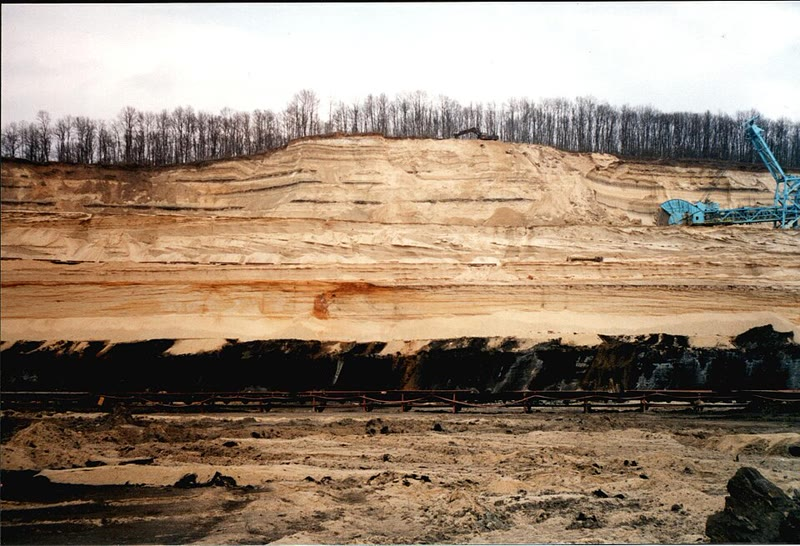
\includegraphics[height=4.0cm]{images/book2/g11-usgs-lignite-bed.jpg}};
\end{tikzpicture}

\medskip
\makebox[0.32\linewidth]{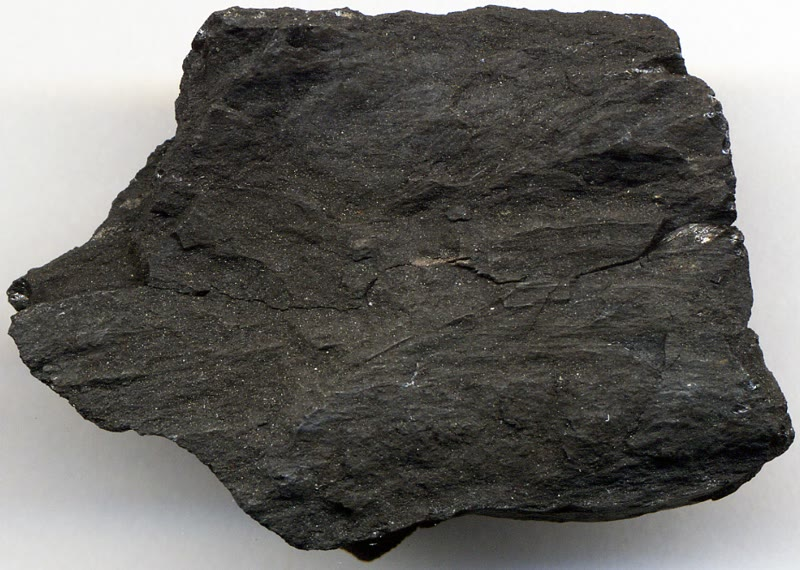
\includegraphics[height=3.2cm]{images/book2/g11-stjohn-lignite.jpg}}\hfill
\makebox[0.32\linewidth]{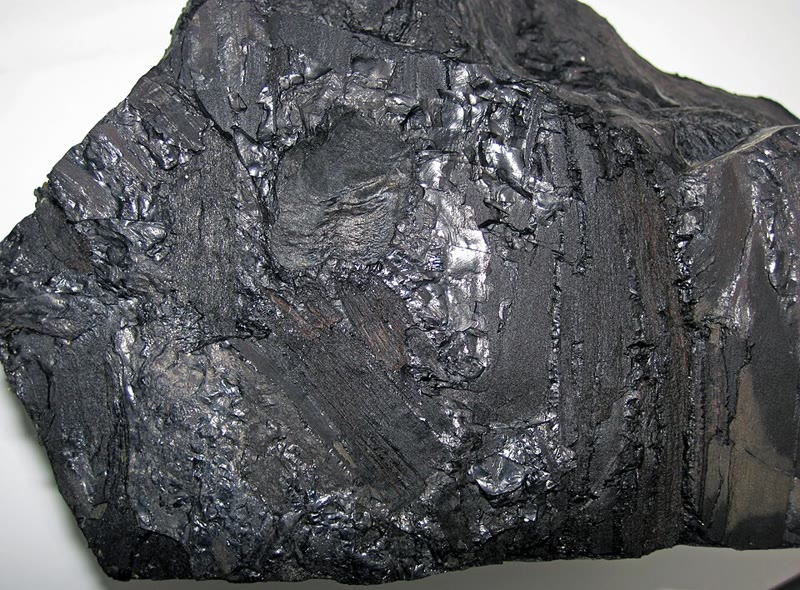
\includegraphics[height=3.2cm]{images/book2/g11-stjohn-bituminous.jpg}}\hfill
\makebox[0.32\linewidth]{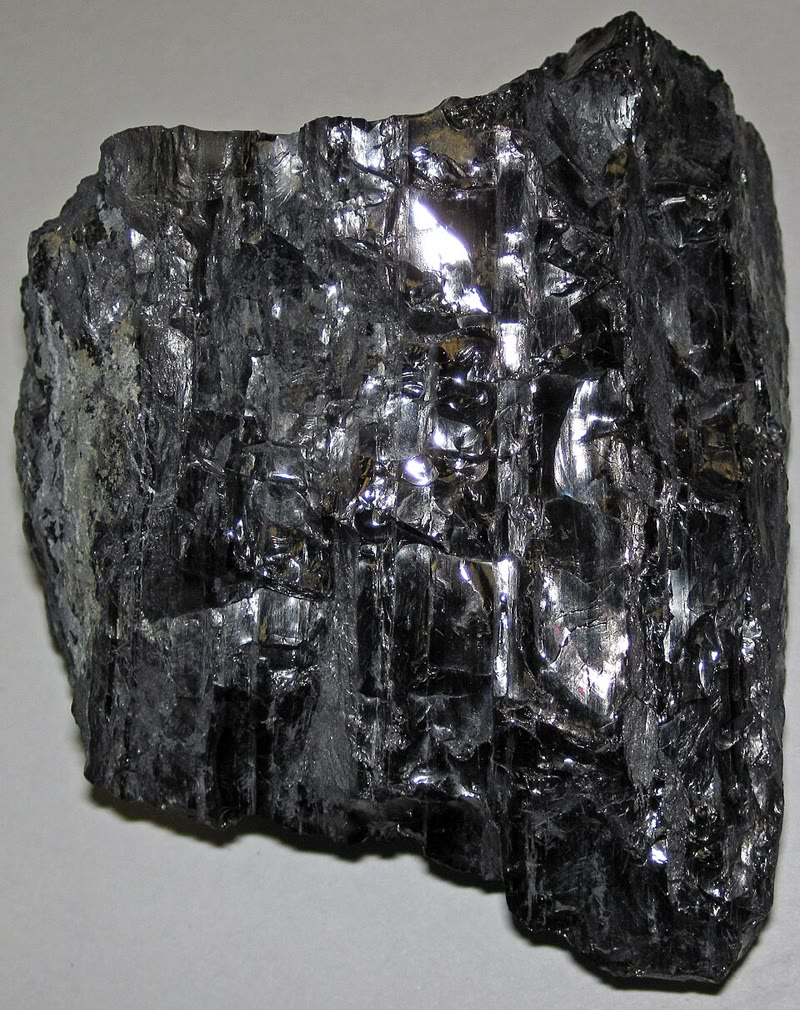
\includegraphics[height=3.2cm]{images/book2/g11-stjohn-anthracite.jpg}}

{\small ऊपर बाएँ: \omterm{def:g11:fossil-fuel-geology:coal}{कोयले} की कोटियों में कार्बन की मात्रा। आँकड़े: अमेरिकी ऊर्जा
सूचना प्रशासन। ऊपर दाएँ: लिग्नाइट की एक परत, हल्की रेत के नीचे
की काली पट्टी, रोमानिया की एक खान में उघड़ी हुई; फ़ोटो अमेरिकी भूवैज्ञानिक
सर्वेक्षण (सार्वजनिक डोमेन)। नीचे, बाएँ से: लिग्नाइट, लगभग \qty{4.5}{cm}
चौड़ा, भूरा-काला और धुँधला; बिटुमिनी \omterm{def:g11:fossil-fuel-geology:coal}{कोयला}, चपटे पौध-अंशों के
साथ; ऐन्थ्रेसाइट, काला और काँच जैसा। फ़ोटो जेम्स सेंट~जॉन
(CC~BY~2.0)।}
\end{omfigure}
% ledger: eia:coal-carbon, photo:g11-lignite-bed, photo:g11-coal-ranks

रास्ते में पीट अपना अधिकांश आयतन खो देता है। मध्य यूटा की एक \omterm{def:g11:fossil-fuel-geology:coal}{कोयला-परत} में,
किसी प्राचीन नदी-धारा द्वारा काटे गए पीट की तुलना उसके बगल में गायब \omterm{def:g11:fossil-fuel-geology:coal}{कोयले} से करने पर
मोटाइयों का अनुपात लगभग $11{:}1$ मिलता है: उस
बिटुमिनी \omterm{def:g11:fossil-fuel-geology:coal}{कोयले} का हर मीटर कभी लगभग ग्यारह मीटर पीट था।
% ledger: ryer80:peat-coal

\section{अभ्यास}

\begin{exercise}[$\star$]\label{exo:g11:fossil-fuel-geology:1}
प्लवक से \omterm{def:g11:fossil-fuel-geology:trap}{ट्रैप} में तेल तक ले जाने वाले चरणों को क्रम में रखिए: \omterm{def:g11:fossil-fuel-geology:migration}{प्रवासन};
\omterm{def:g11:fossil-fuel-geology:oil-window}{तेल-खिड़की} में \omterm{def:g11:fossil-fuel-geology:oil-window}{परिपक्वन}; नए अवसादों के नीचे दफ़न; मृत प्लवक
ऑक्सीजन-विहीन समुद्री तल पर बैठते हैं; तेल \omterm{def:g11:fossil-fuel-geology:reservoir}{आवरण चट्टान} के नीचे इकट्ठा होता है; कार्बनिक
पदार्थ कीचड़ में \omterm{def:g11:fossil-fuel-geology:source-rock}{केरोजन} बन जाता है।
\end{exercise}

\begin{exercise}[$\star$]\label{exo:g11:fossil-fuel-geology:2}
हर चट्टान के लिए बताइए कि वह \omterm{def:g11:fossil-fuel-geology:source-rock}{स्रोत चट्टान}, \omterm{def:g11:fossil-fuel-geology:reservoir}{भंडार चट्टान}
या \omterm{def:g11:fossil-fuel-geology:reservoir}{आवरण चट्टान} होने की अधिक संभावना रखती है: (1) कार्बनिक पदार्थ से समृद्ध गहरे रंग का शेल; (2) जुड़े
छिद्रों वाला सुछँटा बलुआ पत्थर; (3) लवण की एक परत; (4) बिना कार्बनिक
पदार्थ का पंकाश्म; (5) खुले खोखलों से भरा चूना पत्थर।
\end{exercise}

\begin{exercise}[$\star$]\label{exo:g11:fossil-fuel-geology:3}
किसी द्रोणी में सतह \qty{10}{\degreeCelsius} पर है और \omterm{def:g11:lithosphere-asthenosphere:geotherm}{भूतापीय
प्रवणता} \qty{25}{\degreeCelsius/km} है। \omterm{def:g11:fossil-fuel-geology:oil-window}{तेल-खिड़की} किन गहराइयों के बीच
है? वह कितनी मोटी है?
\end{exercise}

\begin{exercise}[$\star$]\label{exo:g11:fossil-fuel-geology:4}
(1) लिग्नाइट, ऐन्थ्रेसाइट, बिटुमिनी \omterm{def:g11:fossil-fuel-geology:coal}{कोयला} और पीट को बढ़ती \omterm{def:g11:fossil-fuel-geology:coal}{कोटि} के क्रम में
रखिए। (2) किसमें कार्बन की मात्रा सबसे अधिक है? (3) कौन-सा सबसे
अधिक गहराई और तापमान पर बना?
\end{exercise}

\begin{exercise}[$\star$]\label{exo:g11:fossil-fuel-geology:5}
(1) \omterm{def:g11:fossil-fuel-geology:trap}{ट्रैप} में गैस तेल के ऊपर, और तेल पानी के ऊपर, क्यों रहता है? (2) भंडार
के ऊपर की चट्टान अपारगम्य क्यों होनी चाहिए? अच्छी \omterm{def:g11:fossil-fuel-geology:reservoir}{आवरण चट्टानें} बनाने वाली दो चट्टानों के नाम
बताइए।
\end{exercise}

\begin{exercise}[$\star\star$]\label{exo:g11:fossil-fuel-geology:6}
दो द्रोणियों का सतही तापमान एक ही है, \qty{15}{\degreeCelsius}।
द्रोणी A की प्रवणता \qty{20}{\degreeCelsius/km} है, द्रोणी B की
\qty{40}{\degreeCelsius/km}। (1) हर एक में \omterm{def:g11:fossil-fuel-geology:oil-window}{तेल-खिड़की} के शीर्ष और आधार की
गहराइयाँ परिकलित कीजिए। (2) दोनों द्रोणियों में एक \omterm{def:g11:fossil-fuel-geology:source-rock}{स्रोत चट्टान} \qty{2}{km} गहराई पर
है। हर एक में वह क्या बनाती है? (3) किस द्रोणी में वहीं बने तेल को पाने के लिए
कुएँ को अधिक गहरा जाना पड़ेगा?
\end{exercise}

\begin{exercise}[$\star\star$]\label{exo:g11:fossil-fuel-geology:7}
मध्य यूटा में किसी पीट की मोटाई और उससे बने \omterm{def:g11:fossil-fuel-geology:coal}{कोयले} की मोटाई के बीच
मापा गया $11{:}1$ का अनुपात लीजिए। (1) \qty{3}{m} मोटी \omterm{def:g11:fossil-fuel-geology:coal}{कोयला-परत} किस मोटाई के पीट
से बनी? (2) मान लीजिए पीट प्रति वर्ष \qty{1}{mm} ढेर हुआ।
उसे इकट्ठा होने में कितना समय लगा? (3) उस पूरे समय दलदल का धँसते रहना
क्यों आवश्यक था?
\end{exercise}

\begin{exercise}[$\star\star$]\label{exo:g11:fossil-fuel-geology:8}
मेरो द्रोणी का दफ़न-इतिहास आरेख उपयोग कीजिए (सतह
\qty{20}{\degreeCelsius}, प्रवणता \qty{30}{\degreeCelsius/km})। \omterm{def:g11:fossil-fuel-geology:source-rock}{स्रोत
चट्टान} 120 मिलियन वर्ष पहले \qty{1.2}{km} गहरी थी, 95
मिलियन वर्ष पहले \qty{2.3}{km} गहरी और 20 मिलियन वर्ष पहले \qty{4.0}{km} गहरी। (1)
हर तिथि पर उसका तापमान परिकलित कीजिए। (2) हर तिथि पर वह अपरिपक्व थी, \omterm{def:g11:fossil-fuel-geology:oil-window}{तेल-खिड़की}
में थी या \omterm{def:g11:fossil-fuel-geology:oil-window}{गैस-खिड़की} में?
\end{exercise}

\begin{exercise}[$\star\star$]\label{exo:g11:fossil-fuel-geology:9}
किसी भंडार बलुआ पत्थर का शीर्ष एक मेहराब बनाता है जिसका शिखर \qty{2400}{m}
गहरा है; उसकी सबसे गहरी बंद समोच्च रेखा \qty{2580}{m} पर है। शिखर पर एक कुआँ
\qty{2450}{m} तक गैस पाता है, फिर तेल। (1) \omterm{def:g11:fossil-fuel-geology:trap}{ट्रैप} जितना स्तंभ रख सकता है,
उसकी अधिकतम ऊँचाई क्या है? (2) यदि \omterm{def:g11:fossil-fuel-geology:trap}{ट्रैप} भरा हो, तो तेल कितना मोटा है?
(3) \omterm{def:g11:fossil-fuel-geology:trap}{ट्रैप} भर जाने के बाद भी आते रहने वाले तेल और गैस कहाँ
जाते हैं?
\end{exercise}

\begin{exercise}[$\star\star$]\label{exo:g11:fossil-fuel-geology:10}
जब \omterm{def:g11:fossil-fuel-geology:source-rock}{केरोजन} का कोई माप उपलब्ध नहीं होता, तो पेट्रोलियम भूवैज्ञानिकों ने
\qty{3}{km} से अधिक चट्टानों के नीचे दबी \omterm{def:g11:fossil-fuel-geology:source-rock}{स्रोत चट्टान} को परिपक्व माना है।
\qty{20}{\degreeCelsius} की सतह के साथ: (1) कौन-सी प्रवणता
\qty{3}{km} को \omterm{def:g11:fossil-fuel-geology:oil-window}{तेल-खिड़की} के शीर्ष पर रखती है? उसके आधार पर? (2) वेध-छिद्रों में मापी गई
25 से \qty{34}{\degreeCelsius/km} की प्रवणताओं के साथ
\qty{3}{km} कहाँ पड़ता है? क्या यह नियम उचित है?
\end{exercise}

\begin{exercise}[$\star\star$]\label{exo:g11:fossil-fuel-geology:11}
\omterm{def:g11:fossil-fuel-geology:coal}{कोयले} के तीन नमूनों में \qty{30}{\percent}, \qty{70}{\percent} और
\qty{92}{\percent} कार्बन है। (1) हर एक की \omterm{def:g11:fossil-fuel-geology:coal}{कोटि} बताइए। (2) पाठ में दी गई
गहराइयों और तापमानों का उपयोग करके बताइए कि कौन-सा सबसे गहरा दबा था?
(3) लिग्नाइट भूरा-काला और धुँधला दिखता है; ऐन्थ्रेसाइट कैसा दिखता है?
\end{exercise}

\begin{exercise}[$\star\star\star$]\label{exo:g11:fossil-fuel-geology:12}
120 और 95 मिलियन वर्ष पहले के बीच मेरो द्रोणी में \qty{1100}{m} कीचड़
ढेर हुआ। (1) दफ़न की दर मीटर प्रति मिलियन वर्ष में परिकलित कीजिए।
(2) \qty{30}{\degreeCelsius/km} की प्रवणता के साथ \omterm{def:g11:fossil-fuel-geology:source-rock}{स्रोत चट्टान} प्रति मिलियन वर्ष कितने डिग्री
गरम हुई? (3) यदि यह दर बनी रहती, तो \omterm{def:g11:fossil-fuel-geology:source-rock}{स्रोत चट्टान} को पूरी \omterm{def:g11:fossil-fuel-geology:oil-window}{तेल-खिड़की} पार करने में
कितना समय लगता? (4) मॉडल लगभग 66 मिलियन वर्ष देता है। अधिक क्यों?
\end{exercise}

\begin{exercise}[$\star\star\star$]\label{exo:g11:fossil-fuel-geology:13}
मेरो द्रोणी में \omterm{def:g11:fossil-fuel-geology:source-rock}{स्रोत चट्टान} लगभग 117 से लगभग 51 मिलियन वर्ष पहले तक
\omterm{def:g11:fossil-fuel-geology:oil-window}{तेल-खिड़की} में थी, और तेल को रोकने वाली अपनति
80 मिलियन वर्ष पहले बनी। (1) मान लीजिए कि खिड़की में रहते हुए \omterm{def:g11:fossil-fuel-geology:source-rock}{स्रोत चट्टान} ने स्थिर दर से
तेल बनाया। उसके तेल का कितना अंश \omterm{def:g11:fossil-fuel-geology:trap}{ट्रैप} के अस्तित्व में आने के बाद
बना? (2) बाक़ी का क्या हुआ? (3) यदि अपनति 40
मिलियन वर्ष पहले बनी होती, तो वह क्या रख सकती थी?
\end{exercise}

\begin{exercise}[$\star\star\star$]\label{exo:g11:fossil-fuel-geology:14}
मेरो द्रोणी का दफ़न-इतिहास लीजिए (\cref{exo:g11:fossil-fuel-geology:8}:
150 मिलियन वर्ष पहले \qty{0.4}{km}, 120 पर \qty{1.2}{km}, 95 पर \qty{2.3}{km},
66 पर \qty{3.0}{km}, बीच में गहराई स्थिर रूप से बढ़ती हुई), पर एक
अधिक गरम द्रोणी: प्रवणता \qty{40}{\degreeCelsius/km}, सतह
\qty{20}{\degreeCelsius}। (1) \omterm{def:g11:fossil-fuel-geology:oil-window}{तेल-खिड़की} के शीर्ष और आधार की
गहराइयाँ परिकलित कीजिए। (2) वे आयु परिकलित कीजिए जिन पर \omterm{def:g11:fossil-fuel-geology:source-rock}{स्रोत चट्टान} खिड़की में प्रवेश करती और
उसे छोड़ती है। (3) अपनति अब भी 80 मिलियन वर्ष पहले बनती है। क्या
वह तेल रखेगी? गैस?
\end{exercise}

\begin{exercise}[$\star\star\star$]\label{exo:g11:fossil-fuel-geology:15}
कार्बोनिफ़ेरस की ऐन्थ्रेसाइट की एक परत अब सतह पर दिखती है।
कार्बोनिफ़ेरस लगभग 299 मिलियन वर्ष पहले समाप्त हुआ। (1) पाठ में दी गई गहराइयों का उपयोग करके बताइए
कि परत कम से कम कितनी गहराई पर दबी थी? (2)
\qty{15}{\degreeCelsius} की सतह और \qty{30}{\degreeCelsius/km} की प्रवणता के साथ
उस गहराई पर वह किस तापमान तक पहुँची? क्या यह ऐन्थ्रेसाइट के लिए दिए गए
तापमान से संगत है? (3) उसके ऊपर पड़ी चट्टानों के साथ क्या हुआ है? यह मानकर कि यह सब
कार्बोनिफ़ेरस के बाद हुआ, औसत दर की, मिलीमीटर प्रति वर्ष में, एक निम्न सीमा बताइए।
\end{exercise}

\section{समस्या: स्रोत चट्टान ने तेल कब बनाया?}

\begin{problem}[{सप्ताहांत समस्या --- एक कल्पित द्रोणी के तेल का काल-निर्धारण}]
\label{pb:g11:fossil-fuel-geology:1}
% values (oil_window.py): enter_oil_Ma 116.97, leave_oil_Ma 51.238, T_max 140, T_today 125,
% after_trap_frac 0.43757; ledger ics:base.Jurassic, ics:base.Cretaceous, earle:*, magoon00:tps
मेरो द्रोणी, एक कल्पित द्रोणी, में किसी अपनति के शिखर से होकर खोदा गया एक कुआँ
नीचे की परतों को पार करता है। अपने जीवाश्मों से दिनांकित, वे
दर्ज करती हैं कि द्रोणी कैसे भरी। सबसे पुरानी से:
\begin{center}
\small
\begin{tabular}{|l|l|l|}
\hline
\textbf{अंतराल (मिलियन वर्ष पहले)} & \textbf{मोटाई} & \textbf{चट्टानें} \\
\hline
165 से 150 & \qty{400}{m} & कार्बनिक पदार्थ से समृद्ध काला शेल, फिर पंकाश्म \\
150 से 120 & \qty{800}{m} & सरंध्र बलुआ पत्थर \\
120 से 95 & \qty{1100}{m} & पंकाश्म \\
95 से 66 & \qty{700}{m} & खड़िया \\
66 से 35 & \qty{700}{m} & रेत और मृत्तिकाएँ \\
35 से 20 & \qty{300}{m} & रेत \\
20 से आज तक & \qty{-500}{m} & उत्थान: ऊपर के \qty{500}{m} अपरदित \\
\hline
\end{tabular}
\end{center}
सतह \qty{20}{\degreeCelsius} पर है और \omterm{def:g11:lithosphere-asthenosphere:geotherm}{भूतापीय प्रवणता}
\qty{30}{\degreeCelsius/km} है, दोनों स्थिर मानी गई हैं। परतें जमने के बाद अपनी
मोटाई बनाए रखती हैं (संहनन की उपेक्षा की गई है)। अपनति 80
मिलियन वर्ष पहले बनी। आधार पर के काले शेल का पीछा कीजिए, जो 165 मिलियन
वर्ष पहले जमा।

\medskip
\noindent\textbf{भाग I --- चट्टानें।}
\begin{enumerate}
  \item कौन-सी परत \omterm{def:g11:fossil-fuel-geology:source-rock}{स्रोत चट्टान} है, कौन-सी भंडार, कौन-सी \omterm{def:g11:fossil-fuel-geology:reservoir}{आवरण चट्टान}?
  \item काले शेल को कार्बनिक पदार्थ से समृद्ध किसने बनाया?
  \item जुरैसिक लगभग \num{201.4} से \num{143.1} मिलियन
        वर्ष पहले तक चला। \omterm{def:g11:fossil-fuel-geology:source-rock}{स्रोत चट्टान} किस कल्प में जमी? और
        बलुआ पत्थर?
  \item \omterm{def:g11:fossil-fuel-geology:source-rock}{केरोजन} क्या है? सतह पर काला शेल कोई तेल क्यों नहीं
        बनाता?
  \item आज \omterm{def:g11:fossil-fuel-geology:source-rock}{स्रोत चट्टान} के ऊपर कितनी मोटाई की चट्टानें पड़ी हैं?
\end{enumerate}

\medskip
\noindent\textbf{भाग II --- समय के सापेक्ष दफ़न।}
\begin{enumerate}[resume]
  \item 150, 120, 95, 66, 35 और 20
        मिलियन वर्ष पहले, और आज, \omterm{def:g11:fossil-fuel-geology:source-rock}{स्रोत चट्टान} की गहराई परिकलित कीजिए।
  \item पहले छह अंतरालों में से हर एक के दौरान दफ़न की दर, मीटर प्रति मिलियन वर्ष में,
        परिकलित कीजिए।
  \item \omterm{def:g11:fossil-fuel-geology:source-rock}{स्रोत चट्टान} सबसे गहरी कब थी, और कितनी गहरी?
  \item पिछले 20 मिलियन वर्षों में उसकी गहराई क्यों घटी?
  \item आज बलुआ पत्थर का आधार कितना गहरा है?
\end{enumerate}

\medskip
\noindent\textbf{भाग III --- समय के सापेक्ष तापमान।}
\begin{enumerate}[resume]
  \item प्रश्न~6 की हर तिथि पर \omterm{def:g11:fossil-fuel-geology:source-rock}{स्रोत चट्टान} का तापमान परिकलित
        कीजिए।
  \item इस द्रोणी में \omterm{def:g11:fossil-fuel-geology:oil-window}{तेल-खिड़की} किन गहराइयों के बीच है?
  \item प्रश्न~6 की किन दो तिथियों के बीच \omterm{def:g11:fossil-fuel-geology:source-rock}{स्रोत चट्टान}
        \qty{60}{\degreeCelsius} से आगे निकली?
  \item यह मानकर कि उस अंतराल में उसकी गहराई स्थिर रूप से बढ़ी, वह आयु परिकलित कीजिए
        जिस पर वह \qty{60}{\degreeCelsius} पर पहुँची।
  \item इसी तरह परिकलित कीजिए कि वह \qty{120}{\degreeCelsius} पर कब पहुँची।
\end{enumerate}

\medskip
\noindent\textbf{भाग IV --- खिड़की में, और ट्रैप।}
\begin{enumerate}[resume]
  \item वह अधिकतम कितने तापमान तक पहुँची? आज वह क्या
        बनाती है?
  \item अपनति के अस्तित्व में आने से पहले बने तेल का क्या हुआ?
  \item यह मानकर कि खिड़की में \omterm{def:g11:fossil-fuel-geology:source-rock}{स्रोत चट्टान} के रहते हुए तेल स्थिर दर से बना,
        उसका कितना अंश अपनति के अस्तित्व में आने के बाद बना?
  \item कुआँ अपनति के शिखर पर किन तरलों की, और ऊपर से किस क्रम में, अपेक्षा
        करेगा?
  \item निष्कर्ष निकालिए: \omterm{def:g11:fossil-fuel-geology:source-rock}{स्रोत चट्टान} ने \omterm{def:g11:fossil-fuel-geology:oil-window}{तेल-खिड़की} में कब प्रवेश किया?
\end{enumerate}
\end{problem}
